\documentclass[../../main]{subfiles}

\begin{document}
\chapter{数ベクトル空間}
\label{chapter:numerical_vector_space}

\begin{lead}
  \cref{chapter:numerical_vector_space}で書く予定のことを並べておく.
\end{lead}

\section{行列と線型空間}
信号解析に関連する議論へと移る前に,有限次元の線型代数について簡単に説明しておく.

\subsection{基底と基底変換}
任意の\(\vect{x}=\trps{\inlinevec{x_1 & \cdots & x_n}}\in\numset{R}^n\)は,第\(i\)成分が\(1\),他の成分が\(0\)のベクトル\(\vect{e}_i\)を用いて
\(\vect{x}=x_1\vect{e}_1+\dots+x_n\vect{e}_n\)と表せる.
すなわち,集合\(\basis{B}_n=\Set{\vect{e}_1,\dots,\vect{e}_n}\)は「\(\numset{R}^n\)のすべての元を\(\basis{B}_n\)の元の線型結合で書ける」という性質を持つ.

一般に,線型空間\(V\)の部分集合\(S\)に対して,\(S\)の元の線型結合で書けるベクトルの全体集合を\(S\)が\termdef{生成する部分空間}\index{ぶぶんくうかん@部分空間!せいせいする@生成する---}(generated subspace)といい,
\(\spannedby S\)と表記する.この言葉を使えば,先述した\(\basis{B}_n\)が持つ性質は「\(\spannedby\basis{B}_n=\numset{R}^n\)が成り立つ」とも言い換えられる.

\(\spannedby S=\numset{R}^n\)を満たす集合\(S\subset\numset{R}^n\)は,\(\basis{B}_n\)以外にも無数にある.
たとえば\(n=2\)のとき,集合\(S=\Set{\trps{\inlinevec{1 & 1}},\trps{\inlinevec{2 & -1}},\trps{\inlinevec{-1 & 0}}}\)が生成する部分空間は
\(\numset{R}^2\)である.しかし,\(\basis{B}\)の線型結合で\(\numset{R}^2\)の元を表す方法はただ1通りであるのに対して,\(S\)はこの性質を持たない.

\begin{figure}[htbp]
  \centering
  \begin{minipage}{0.5\linewidth}
    \centering
    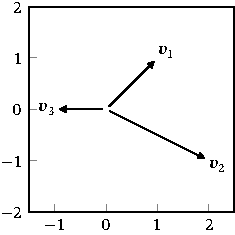
\includegraphics{linear_comb1.pdf}
  \end{minipage}%
  \begin{minipage}{0.5\linewidth}
    \centering
    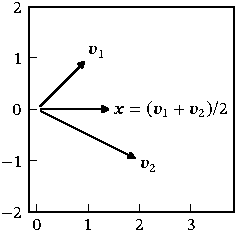
\includegraphics{linear_comb2.pdf}    
  \end{minipage}
  \caption{\(S\)の元の線型結合で\(\vect{x}=\trps{\begin{bmatrix}3/2 & 0\end{bmatrix}}\)を表した様子.明らかに\(\vect{x}=(-3/2)\vect{v}_3\)と表せるが,一方で\(\vect{x}=(\vect{v}_1+\vect{v}_2)/2\)も成り立つ.}
\end{figure}

\subsection{固有値と固有空間}
\begin{definition}{固有値,固有空間}{eigenvalue}\index{こゆうち@固有値}\index{こゆうべくとる@固有ベクトル}
\(\mat{A}\)を\(n\)次正方行列とする.
複素数\(\lambda\)と\(\zvec\)でないベクトル\(\vect{x}\in\numset{C}^n\)が式\(\mat{A}\vect{x}=\lambda\vect{x}\)を満たすとき,
\(\lambda\)を\(\mat{A}\)の\termdef{固有値}(eigenvalue)という.
また,\(\vect{x}\)を\(\mat{A}\)の(固有値\(\lambda\)に属する)\termdef{固有ベクトル}(eigenvector)という.
\end{definition}

\begin{definition}{固有空間}{eigenspace}\index{こゆうくうかん@固有空間}
\cref{definition:eigenvalue}の\(\mat{A}\),\(\lambda\)について,集合
\[
  E_\lambda(\mat{A}) = \Set{\vect{x}\in\numset{C}^n\given\mat{A}\vect{x}=\lambda\vect{x}}
\]
は\(\numset{C}^n\)の部分空間になる.部分空間\(E_\lambda(\mat{A})\)を,
\(\mat{A}\)の(固有値\(\lambda\)に属する)\termdef{固有空間}(eigenspace)という.
\end{definition}

固有空間は次の性質を持つ.

\begin{proposition}{}{eigenspaces_disjointness}
\(\lambda_1\),\(\lambda_2\)を\(n\)次正方行列\(\mat{A}\)の固有値とする.
\begin{enumerate}
  \item \(\vect{x}\in E_{\lambda_1}(\mat{A})\implies\mat{A}\vect{x}\in E_{\lambda_1}(\mat{A})\)
  \item \(\lambda_1\neq\lambda_2\implies E_{\lambda_1}(\mat{A})\cap E_{\lambda_2}(\mat{A})=\Set{\zvec}\)
\end{enumerate}
\end{proposition}

\subsection{対角化}

\section{直交射影}
\subsection{直交射影}
\subsection{直交補空間}
\subsection{スペクトル定理}

\section{最小二乗問題}
\subsection{最小二乗問題}
\subsection{特異値分解}
\subsection{擬似逆行列}

\section{離散フーリエ変換}

\section{多重解像度解析}

\begin{subappendices}
\section{主成分分析}
\section{低ランク近似}
\section{窓関数}
\end{subappendices}

\section*{演習問題}
\addcontentsline{toc}{section}{演習問題}

\end{document}
